\documentclass{beamer}
\usepackage{graphicx}
\usepackage{hyperref}
\title{CPP Community Garden Meeting Note}
\author{An Pham, Myriam, Tyler, Melvin, Kayla, Chris}
\institute{Calpoly Pomona}
\date{\today}
\usetheme{Boadilla}
%\usetheme{Berkeley}
\usepackage{graphicx}
\usepackage{booktabs}
\usepackage{hyperref}
\usepackage{subfig}
\usepackage[english]{babel}

\begin{document}
\frame{\titlepage}

\begin{frame}
\frametitle{Overview}
\begin{enumerate}
  \item Report conceptual design.
  \item Revisition AWS IoT Core Services.
  \item Describe the Soil Sensors (LORA version).
  \item Publish and Discuss bill of material for lab environment.
  \item Establish the challenges as well as problem while implementing new tech stack.
 \end{enumerate}
\end{frame}

\begin{frame}
 \frametitle{Recape the hardware in the Project}
   \begin{itemize}
    \item Problem:
      \begin{itemize}
       \item Most of soil moisture sensors fail.
       \begin{itemize}
         \item losing connection.
	 \item inconsistent of uptime.
	 \item can't operate in outdoor environment.
       \end{itemize}
       \item Soil dryness.
      \end{itemize}
    \item Need: 
    \begin{itemize}
      \item How to detect dryness and maintain the wetness of the garden soil?
      \item A type of soil sensors technology that is reliable.
    \end{itemize}
   \end{itemize}
\end{frame}

\begin{frame}
  \frametitle{AWS with Lora and non-Lora System}
  \begin{figure}[h]
  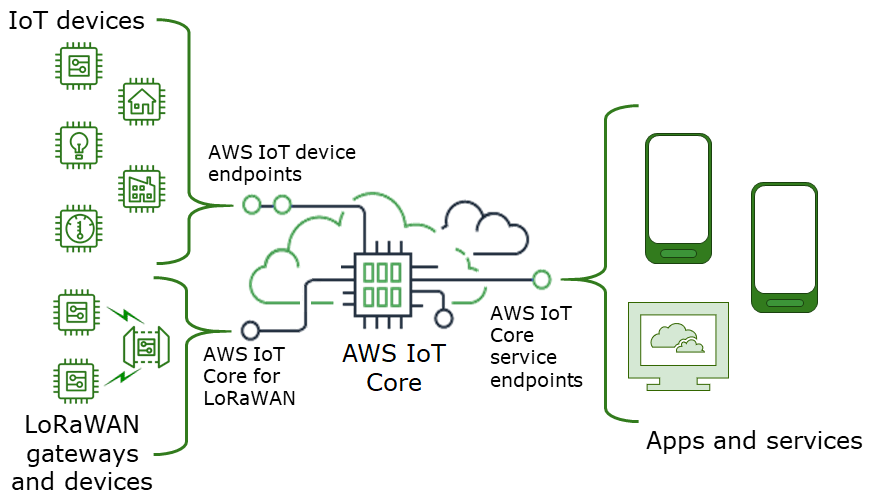
\includegraphics[scale=0.5]{iot-endpoints.png}
    \caption{AWS IoT Core Overview (Source: AWS)}
\end{figure}

\end{frame}

\begin{frame}[t]
  \frametitle{IoT HUb}
  \begin{itemize}
    \item What Software Included:
      \begin{enumerate}
        \item AWS LoRa Basics Station - https://github.com/lorabasics/basicstation.
	\item ecowitt2mqtt - https://github.com/bachya/ecowitt2mqtt  
      \end{enumerate}
  \end{itemize}
  \begin{itemize}
    \item AWS LoRA Basic Station is used to forward lora signal to AWS IoT Core.
    \item ecowitt2mqtt is used to forward mqtt signal to AWS IoT Core.
  \end{itemize}
\end{frame}

\begin{frame}[t]
  \frametitle{Lora Moisture Sensors}
  \begin{figure}
      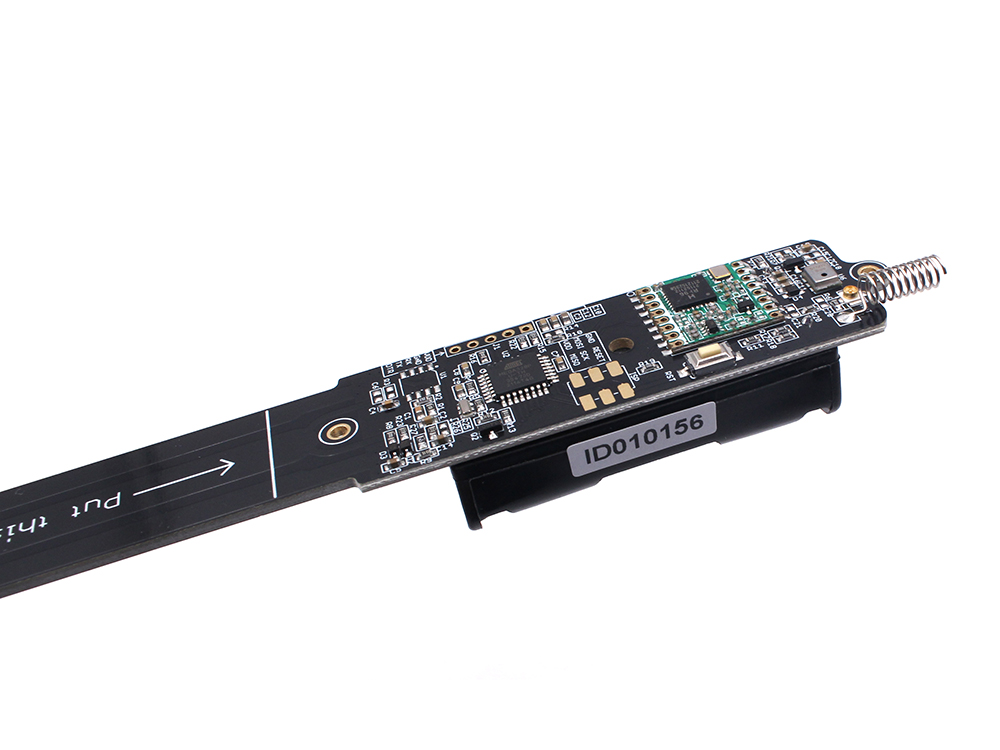
\includegraphics[width=.2\textwidth]{Lora-Soil-Moisture-V3-3-1000x750.jpg}
      \hfill 
      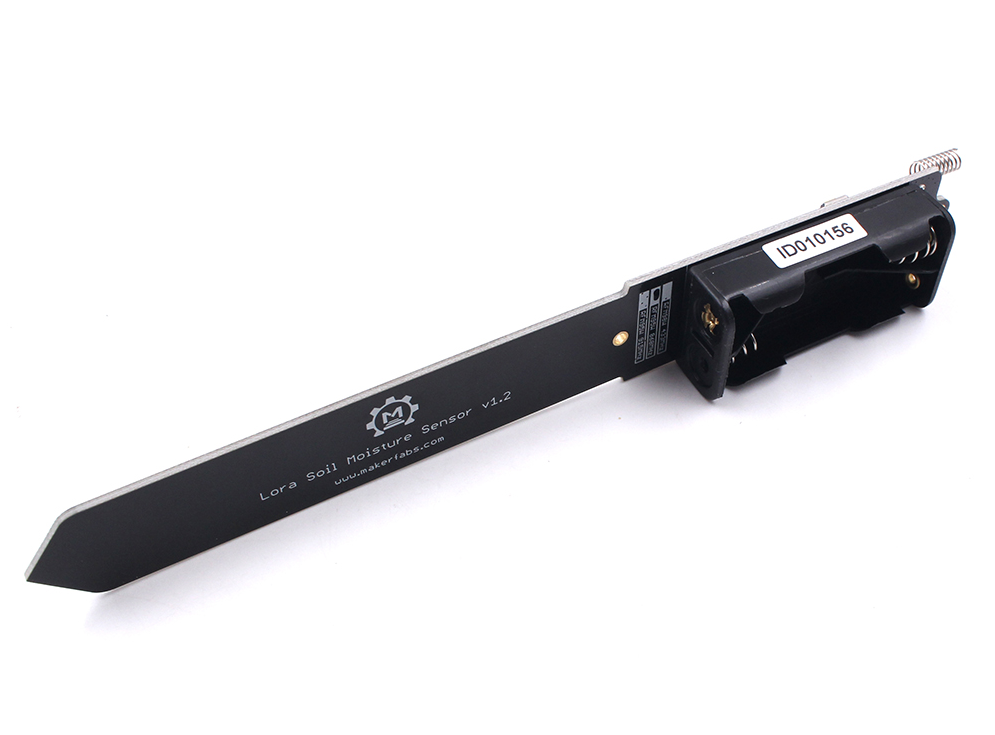
\includegraphics[width=.2\textwidth]{soil-moisture-sensors.png} 
      \hfill
      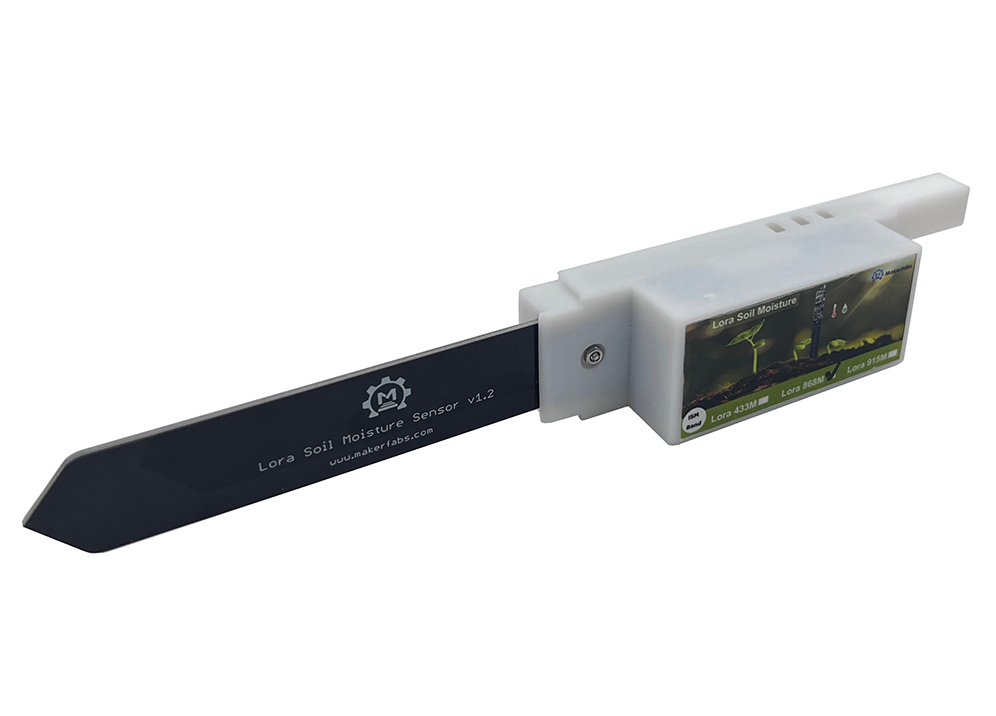
\includegraphics[width=.2\textwidth]{soil-moisture-sensors2.png}
      \hfill

    \end{figure} 

  \begin{itemize}
    \item Refer for completion of the project: https://www.makerfabs.com/lora-soil-moisture-sensor-v3.html 
  \end{itemize} 
\end{frame}

\begin{frame}[t]
 \frametitle{Agenda (reviewed on Aug 15)}
 \begin{itemize}
   \item Discuss with Melvin and Myriam regarding DIY gateway solution and Implementing AWS IoT Core
     \begin{itemize}
       \item IoT can aggregate the signal sent from devices. 
       \item Address the previous of Melvin's Research on Greengrass. 
	 \begin{itemize}
	   \item What features we need on Greengrass?
	   \item Can the functions performed remotely?
	 \end{itemize}
     \end{itemize}
   \item Decide the prototype for Product Demo in Fall 2023 presentation.
     \begin{itemize}
       \item Outcome: Able to set up LORA soil moisture sensors along with AWS iot Core.
     \end{itemize}
 \end{itemize} 
\end{frame}


\begin{frame}[t]
  \frametitle{Reference }
  \framesubtitle{Sources}
 \begin{itemize}
    \item \url{https://docs.aws.amazon.com/iot/latest/developerguide/connect-to-iot.html} {LORA and Non-LORA AWS IoT Core}.
    \item \url{https://github.com/lorabasics/basicstation} {BasicStation}.
    \item \url{https://docs.aws.amazon.com/iot/latest/developerguide/connect-to-iot.html}.
    \item \url{https://www.makerfabs.com/lora-soil-moisture-sensor-v3.html}.
 \end{itemize}
\end{frame}


\end{document}
